\section{Query-based Architecture}
Recently, query-based architectures have achieved marvelous success in most computer vision tasks such as object detection \cite{carion_end--end_2020}, object tracking \cite{meinhardt_trackformer_2022}, and image segmentation \cite{cheng_masked-attention_2022, cheng_per-pixel_2021}. The main component in these architectures is a Transformer model with a set of object queries. 

\vspace{-2mm}
DETR \cite{carion_end--end_2020} introduced the new query-based paradigm for object detection. The image features were encoded by a transformer encoder, then these encoder output were used to transform a set of object queries into the output embedding by the decoder. 

\vspace{-2mm}
An extension of this method for Video Instance Segmentation(VIS) was presented in VisTR. Wang et al. \cite{wang_end--end_2021} proposed a new strategy of instance sequence matching and segmentation to simultaneously supervise and segment instances at the sequence level (Figure \ref{fig:vistr}). 

\begin{figure}[b!]
    \centering
    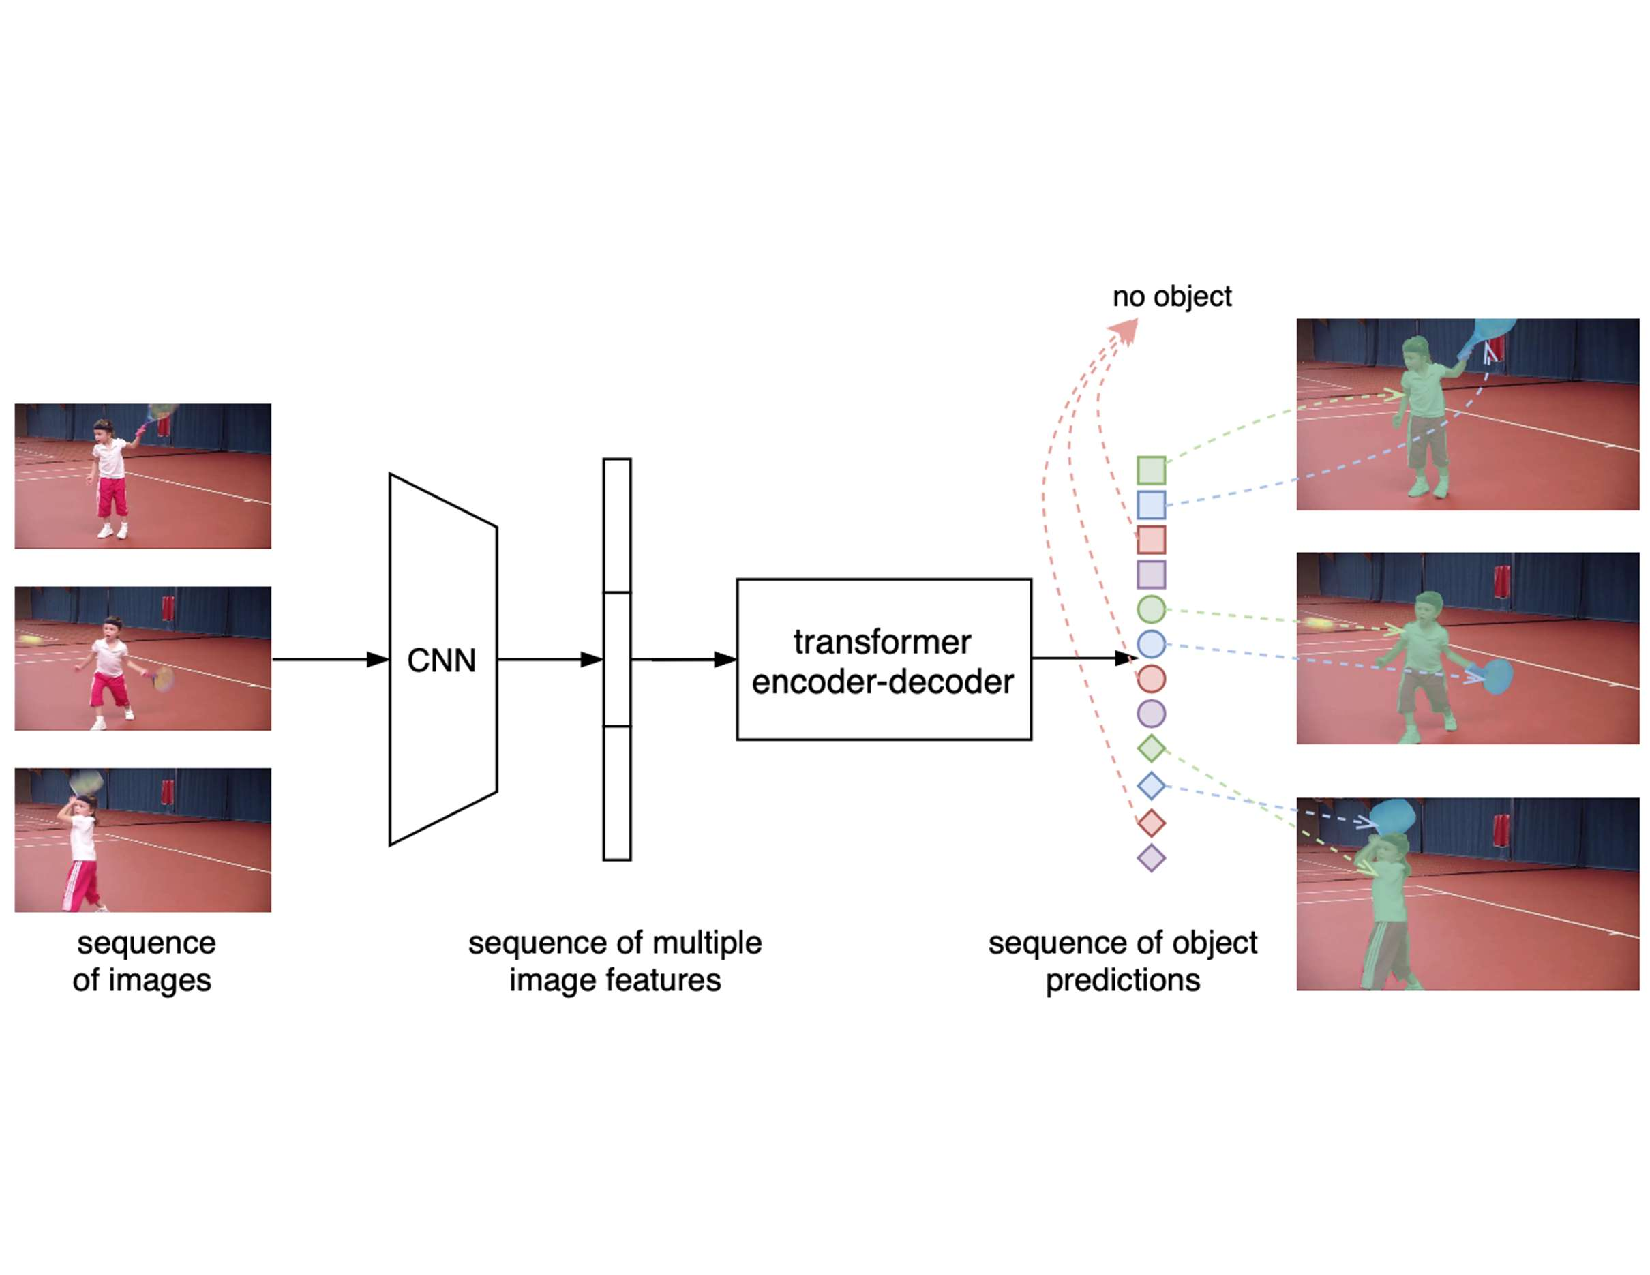
\includegraphics[width=\textwidth]{content/resources/images/VisTR.pdf}
    \caption{The overall architecture of VisTR \cite{wang_end--end_2021} }
    \label{fig:vistr}
\end{figure}

\vspace{-2mm}
MaskFormer \cite{cheng_per-pixel_2021} introduced the new mask classification instead of the per-pixel classification for segmentation tasks. By using a set of queries as, MaskFormer shows the simple and convenient for the general segmentation paradigm.\\ Mask2Former \cite{cheng_masked-attention_2022} extended the meta-architecture of MaskFormer with a new Masked-attention transformer decoder and utilized high-resolution features to handle objects on multiple scales. Mask2Former finally sets a new state-of-the-art in all three major image segmentation tasks (panoptic, instance and semantic) while remaining easy to train. 


% In this work, we utilize the powerful architecture from Mask2Former to capture the multi-scale visual features, which then are associated with linguistic 
